%!TEX TS-program = xelatex
%!TEX encoding = UTF-8 Unicode
%!BIB TS-program = biber
%!BIB program = biber

\documentclass[xetex,compress,spanish,tikz]{beamer}

%\setbeameroption{show notes}
%\usepackage{pgfpages}\setbeameroption{show notes on second screen}
%\setbeameroption{show only notes}
\setbeameroption{hide notes}

\mode<presentation>
{
  \usetheme{Warsaw}
  \usecolortheme[rgb={.7,.2,.2}]{structure}
  \setbeamercovered{transparent}
}
\useoutertheme[footline=authortitle,subsection=false]{miniframes}

\usepackage[no-math]{fontspec}
\usepackage[spanish,es-tabla,es-noshorthands,es-ucroman]{babel}
\usepackage{xltxtra}
\usepackage{fontspec}
\usepackage{xunicode}
\usepackage{amsmath}
\usepackage{amsthm}
\usepackage{graphicx}
\usepackage{amssymb}
\usepackage{hyperref}
\usepackage{siunitx}
\usepackage{tikz}
\usetikzlibrary{calc}
\usepackage{booktabs}
\usepackage{subfigure}
\usepackage{csvsimple}
\usepackage[colorinlistoftodos, shadow]{todonotes}
  \presetkeys{todonotes}{inline}{}

%% bib %%
\usepackage[style=authoryear,natbib=true,%
maxbibnames=99,maxcitenames=2,%
citestyle=authoryear-comp,doi=true,url=true,backend=biber,dashed=no]{biblatex}
\bibliography{pfc-memoria.bib}
%% style %%
\defaultfontfeatures{Mapping=tex-text,Numbers={OldStyle}}
\setmainfont[Mapping=tex-text]{Hoefler Text}
\setromanfont[Mapping=tex-text]{Hoefler Text}
\setsansfont[Scale=MatchLowercase,Mapping=tex-text]{Gill Sans}
\setmonofont[Scale=0.9]{Courier New}
\sisetup{output-decimal-marker={,},
	product-units=single,
	detect-all, detect-inline-family=text, detect-inline-weight=text,
  detect-display-math=true}

%% custom macros %%
\newcommand{\email}[1]{%
  \href{mailto:#1}{\nolinkurl{<#1>}}}

\DeclareSIUnit[number-unit-product = {\,}]
	\pixel{px}

%% doc info %%
\title{Procesamiento del Lenguaje Natural Aplicado al Análisis del Sentimiento de Opiniones}
\author[Guillermo Gutiérrez-Herrera]{Proyecto Fin de Carrera\\Ingeniero en Informática (Plan 97)\\[1em]
Realizado por: Guillermo Gutiérrez-Herrera\\[1em]
Dirigido por: José Antonio Troyano}
\institute{Departamento de Lenguajes y Sistemas Informáticos\\
Escuela Técnica Superior de Ingeniería Informática\\
Universidad de Sevilla}
\date{Septiembre de 2015}
\logo{
\includegraphics[width=10pt]{logo-lsi}\hspace{2pt}
\includegraphics[width=15pt]{logo-us}}
\subject{Procesamiento de NLP aplicado al Análisis de Sentimiento}
\keywords{Natural Language Processing, Machine Learning, Sentiment Analysis}


\expandafter\def\expandafter\insertshorttitle\expandafter{%
  \insertshorttitle\hfill%
  \insertframenumber\,/\,\inserttotalframenumber}
  
%% documento %%
\begin{document}

\frame{
\titlepage

\tikz[overlay,remember picture]
\node[anchor=center] at ($(current page.south west)+(1.3,1.3)$) {

\includegraphics[width=40pt]{logo-us}
};

\tikz[overlay,remember picture]
\node[anchor=center] at ($(current page.south west)+(2.9,1.3)$) {

\includegraphics[width=30pt]{logo-lsi}
};

\note{[Buenos días] / [Buenas tardes]. Mi nombre es Guillermo Gutiérrez y voy a presentar mi Proyecto Fin de Carrera titulado \emph{Procesamiento del Lenguaje Natural Aplicado al Análisis del Sentimiento de Opiniones} y dirigido por el profesor José Antonio Troyano.}
}

%\section[Índice]{}
\frame{\frametitle{Índice}
\tableofcontents

\note[item]<1>{Empezaremos la presentación con una breve introducción y los objetivos del proyecto; y la planificación y metodología utilizados para su realización.}
\note[item]<1>{En la siguiente parte resumiremos los métodos de Procesamiento de Lenguaje Natural y las técnicas de Aprendizaje Automático que se describen en la memoria.}
\note[item]<1>{A continuación presentamos el problema concreto de clasificación automática del sentimiento; y el diseño de la solución propuesta.}
\note[item]<1>{Y por último las conclusiones del proyecto y la bibliografía que se ha usado principalmente para la realización de este proyecto.}
}

\section[Introducción]{Introducción y objetivos}

\frame{\frametitle{Introducción}
\begin{itemize}
\item Los compiladores, traductores y procesadores de lenguajes tradicionales procesan \textbf{lenguajes formales.}
\item El lenguaje formal se diseña formalmente para evitar la ambigüedad.
\item El \textbf{lenguaje natural} es ambiguo por naturaleza.
\item Dentro del ámbito de la Inteligencia Artificial, se ha comprobado eficaz aplicar Aprendizaje Automático al tratamiento del lenguaje natural.
\item En este proyecto:
\begin{itemize}
\item Se resumen estas técnicas.
\item Se desarrolla una aplicación gráfica para usar como laboratorio de experimentación.
\end{itemize}
\end{itemize}
}

\frame[plain]{\frametitle{Introducción. Explosión de información digital}
\centering
\pgfimage[height=0.98\textheight]{Hilbert-InfoGrowth}
\nocite{Hilbert2011}

\note[item]<1>{En el artículo de \citep{Hilbert2011} titulado \citetitle{Hilbert2011} se realiza una estimación de la capacidad global de almacenamiento en los últimos años.}
\note[item]<1>{En el gráfico podemos observar un incremento exponencial a partir del año 2002 cuando Internet comienza a ser un elemento imprescindible en la mayoría de hogares.}
\note[item]<1>{Esto demuestra la posibilidad real de aplicar herramientas de tratamiento automático de la información para sintetizar el conocimiento; en el caso de procesar información textual: se puede extraer conocimiento sobre los propios lenguajes (morfología, sintaxis, gramática, semántica), sin que tenga un coste excesivo pues existe gran cantidad de datos disponible en Internet gratuitamente, tan sólo hay que recogerlo y ordenarlo.}
}

\frame{\frametitle{Introducción. Polaridad del sentimiento}
\begin{definition}[Polaridad del sentimiento]
Es la conclusión que se extrae de la comprensión de un documento de tipo crítico: si el objeto de la crítica es bueno (sentimiento positivo) o malo (resp., negativo).
\end{definition}
\begin{figure}[htbp]
\centering
\pgfimage[height=0.47\textheight]{tramos-polaridad}
\caption{Escala de valoración del sentimiento usada en Penn Sentiment Treebank de la Universidad de Pennsylvania \citep{Socher2014}}
\end{figure}

\note[item]<1>{\fullcite{Socher2014}}
\note[item]<1>{... Comentar sobre reputación de marcas, análisis en twitter, ...}
}

\frame{\frametitle{Objetivos}
Los objetivos del proyecto son
\begin{itemize}
\item Estudiar
\begin{itemize}
\item Diferencias entre el lenguaje natural y formal.
\item Estrategias, métodos, procedimientos y algoritmos para analizar y extraer información de textos en lenguaje natural (NLP).
\item Algoritmos de aprendizaje automático (ML).
\end{itemize}
\item Desarrollar
\begin{itemize}
\item Biblioteca unificada de NLP y ML para el análisis del sentimiento.
\item Aplicación gráfica para usar en el aula.
\end{itemize}
\end{itemize}
}

\section[Planificación]{Planificación y metodología}

\frame[plain]{%\frametitle{Planificación. Listado de tareas}
\centering
\begin{minipage}{0.71\textwidth}
\resizebox{0.86\textheight}{!}{\csvautotabular{gantt.csv}}
\end{minipage}
\begin{minipage}{0.25\textwidth}
\begin{tabular}{c|c}
\toprule
Estimado & 561 horas\\
Real & 625 horas\\
\bottomrule
\end{tabular}
\end{minipage}
}

\frame[plain]{%\frametitle{Planificación. Diagrama de Gantt}
\tikz[overlay,remember picture]
\node[anchor=north west] at ($(current page.north west)+(-10pt,-5pt)$) {
  \pgfimage[width=1.03\paperwidth]{gantt}
};
}

\frame{\frametitle{Metodología de trabajo}
\begin{figure}[htbp]
\centering
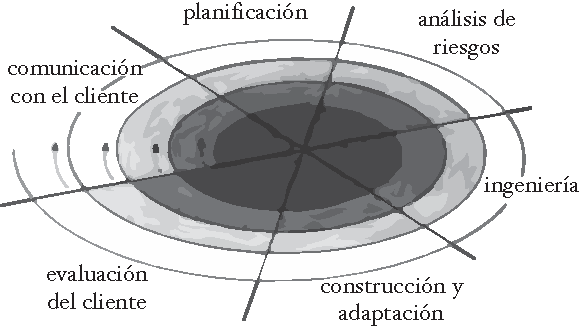
\includegraphics[width=0.58\textwidth]{espiral}
\caption[Modelo de ciclo de vida en espiral]{Modelo de ciclo de vida en espiral \citep{Boehm1988}}
\label{fig:espiral}
\end{figure}
}

\section[NLP]{Procesamiento del Lenguaje Natural}

\frame{\frametitle{Procesamiento del Lenguaje Natural}
\todo{Diferencias entre lenguaje natural, artificial, construido ...}
\todo{Nombrar ejemplo STUDENT (Bobrow1964) ...}
\todo{Nombrar Linguistic Data Consortium, forma de trabajar con datasets ...}
}

\frame{\frametitle{NLP. Preprocesamiento}
\todo{transformaciones / filtros}
\todo{tokenización, stopwords, stemming (nombrar Porter), lemmatizing, anotación POS-tagging ...}
}

\frame{\frametitle{NLP. Análisis}
\todo{analisis sintáctico, ...}
\todo{modelo de espacio vectorial semántico, ...}
}



\section[ML]{Aprendizaje Automático}

\frame{\frametitle{Aprendizaje automático}
\todo{definición}
\todo{ejemplos de utilidad}
}

\frame{\frametitle{ML. Tipologías}
\todo{Definir las 3 clases y enumerar ejemplos de algoritmos, ...}
\todo{supervisado, ...}
\todo{no supervisado, ...}
\todo{semi-supervisado, ...}
}

\frame{\frametitle{ML. Espacio de características}
\todo{figura espacio de características }
}

\frame{\frametitle{ML. Extracción de características}
\todo{BOW, 2-BOW, n-BOW,... }
\todo{RNN, (Socher2013), ... }
\todo{VM-RNN, (Socher2013), ... }
}

\frame{\frametitle{ML. Reducción de características}
\todo{umbral de varianza, ...}
}

\frame{\frametitle{ML. Bondad del estimador}
\todo{precision, recall, f-value, ...}
}

\frame{\frametitle{ML. Estimadores (I)}
\todo{enumerar NB multinomial, NB gausiano, discriminantes LDA/QDA,}
}

\frame{\frametitle{ML. Estimadores (y II)}
\todo{SVM, poner figura 4.10 }
}

\section{Problema}

\frame{\frametitle{Problema a resolver}
\todo{Definición del problema de Kaggle - rotten tomatoes, ...}
}

\section[Diseño]{Diseño de la solución}

\frame{\frametitle{Diseño de la solución}
\todo{Diagrama casos de uso (fig 5.1)}
}

\frame{\frametitle{Diseño. Patrón de diseño}
\todo{figura MVC y figura MVP (6.1)}
}

\frame{\frametitle{Diseño. Arquitectura de componentes}
\todo{figura 6.2}
}

\frame{\frametitle{Diseño. Toolkits de desarrollo GUI}
\todo{Comentar Kivi, comentar QML(Qt)}
}

\frame{\frametitle{Diseño. Pantallas}
\todo{un par de screenshots  de la app (figs tomadas del capítulo manual de usuario de la memoria)}
}


\section[Conclusiones]{Conclusiones y continuidad}

\frame{\frametitle{Conclusiones}
\todo{capitulo Conclusiones de la memoria ... }
}

\frame{\frametitle{Posibles mejoras}
\todo{capitulo Trabajo futuro de la memoria ... }
}

\section{Bibliografía}

\frame{\frametitle{Bibliografía}
\todo{Completar...}
\printbibliography[title=\bibname]
}
%\newrefcontext para dividir citas
% Hilbert2011
% Socher2014
% Boehm1988

\appendix

\frame{
\Huge ¿Preguntas?
\tikz[overlay,remember picture]
\node[anchor=center] at ($(current page.center)+(2,0)$) {
  
\includegraphics[width=120pt]{preguntas}
};
}

\frame{
\centering
\huge Gracias por su atención

\vspace{0.2\textheight}

\normalsize
\begin{minipage}{5.3cm}
Guillermo Gutiérrez-Herrera

\email{guiguther@alum.us.es}

\email{xiterrex@gmail.com}
\end{minipage}
}

\end{document}
